\documentclass[a4paper,12pt]{article}
%\documentclass[a4paper,10pt]{scrartcl}

\usepackage{scrextend}
\changefontsizes[14pt]{14pt}

\usepackage[T1]{fontenc}
\usepackage{lmodern}
\usepackage[utf8x]{inputenc}
\usepackage{graphicx}
\usepackage{tabularx}
\usepackage{multirow}
\usepackage{booktabs}
\usepackage{colortbl}
\usepackage[italian]{babel}
\usepackage[margin=2cm]{geometry}
\usepackage{color}
\definecolor{mygrey}{gray}{0.4}
\definecolor{light-blue}{rgb}{0.4,0.5,1}
\definecolor{light-cyan}{rgb}{0.4,0.6,1}
\usepackage{booktabs}


%Header and footer of pages
\usepackage{fancyhdr}
\pagestyle{fancy}
\lhead{\textcolor{mygrey}{Emanuele Uliana, Gabriele Rufolo, Walter Rubino}}
\rhead{\textcolor{mygrey}{RASD}}

%Set paragraphs indentation to 0 points
\setlength{\parindent}{0pt}

%Sections and subsections' style
\usepackage{titlesec} 
\titleformat{\section} {\color{blue}\normalfont\sffamily\Large\bfseries} {\color{blue}\thesection}{20pt}{} 
\usepackage{titlesec}
\titleformat{\subsection} {\color{light-blue}\normalfont\sffamily\large\bfseries\itshape} {\color{light-blue}\thesubsection}{18pt}{} 
\titleformat{\subsubsection} {\color{light-cyan}\normalfont\sffamily\large\bfseries\itshape} {\color{light-cyan}\thesubsubsection}{14pt}{} 

%Document default font family
\renewcommand{\familydefault}{\sfdefault}
\renewcommand*\arraystretch{1.5}

\pdfinfo{%
  /Title    (SWIMv2 - RASD)
  /Author   (Emanuele Uliana /and Gabriele Rufolo / and Walter Rubino)
  /Creator  (Emanuele Uliana /and Gabriele Rufolo / and Walter Rubino)
  /Producer (Emanuele Uliana /and Gabriele Rufolo / and Walter Rubino)
  /Subject  (RASD)
  /Keywords ()
}

\begin{document}
\vspace*{\fill}
\begin{center}
{\fontsize{28}{10} \selectfont \textcolor{mygrey}{Progetto di Ingegneria del Software 2} \\[2\baselineskip]} {\fontsize{42}{10} \selectfont {\bfseries SWIMv2}} \\[4\baselineskip]

\includegraphics[scale=0.4]{polimi} \\[4\baselineskip]
{\fontsize{28}{10} \selectfont {\bfseries \textcolor{blue}{Requirements Analysis Specification Document}} \\[2\baselineskip] A.A. 2012/2013}
\end{center}
\begin{flushleft}
{\fontsize{18}{10}
{\bfseries Autori}: \\ Emanuele Uliana (799256), Gabriele Rufolo (743695), Walter Rubino (742519) \\[1\baselineskip]
{\bfseries Docente}: \\ Prof.ssa Raffaela Mirandola
}
\end{flushleft}
\vspace*{\fill}
\begin{center}
Versione 1.1 del 12/12/2012 \\
\end{center}

\clearpage

	    \vspace*{\fill}
	\tableofcontents
	    \vspace*{\fill}

\clearpage

\section{Descrizione}
Si vuol sviluppare un social network che consenta agli utenti di aiutarsi reciprocamente inviando richieste di supporto e/o fornendo egli stesso aiuto. \\ \\
L’utente non registrato (ospite) ha la sola facoltà di lettura dei quesiti, delle risposte e delle soluzioni ma senza possibilità di interagire con alcuno dei soggetti interessati. \\ \\
Il sistema deve permettere la creazione di nuovi utenti tramite l’immissione di credenziali di accesso quali l’email e la password. Una volta registrato l’utente potrà non solo leggere le risposte ai problemi già noti (pubblicati da terzi) ma anche contribuire sia alla soluzione del problema sia ponendo nuove domande. \\ \\
Il sistema implementa anche un sistema di gestione dei feedback con il quale è possibile valutare l’operato di chi ha fornito aiuto creando così un forte ed efficiente sistema di collaborazione. \\ \\
I quesiti possono essere posti sia in privato tramite l’utilizzo di messaggi privati tra due utenti che immissione di domande nella bacheca pubblica e quindi visibile da tutti gli internauti (anche ai non registrati, vedi sopra).

\clearpage

\section{Introduzione}
\subsection{Glossario}
Al fine di migliorare la comprensione del seguente documento si riportano qui sotto alcune tra le principali definizioni dei termini usati all’interno dello stesso:
\begin{itemize}
\itemsep0em
\item {\bfseries Abilità}:
è un abilità posseduta dall’utente e può riferirsi ad esempio a conoscenze in ambito culinario, sportivo, professionale, accademico, scolastico, hobbistico etc.
\item {\bfseries Account}: vedi \textit{profilo}
\item {\bfseries Argomento}: vedi \textit{thread}
\item {\bfseries Bacheca}:
con bacheca intendiamo l’insieme totale dei messaggi pubblici presenti sulla piattaforma SWIMv2
\item {\bfseries Messaggio privato}:
è uno strumento che consente agli utenti di inviarsi messaggi tra loro privatamente per chiedere aiuto e/o rispondere a richieste di aiuto ricevute
\item {\bfseries Feedback}:
è la possibilità di esprimere un giudizio sull’operato di un utente
\item {\bfseries Post}:
è il singolo messaggio scritto da un utente, esso può contenere un domanda, un messaggio di risposta o anche una soluzione
\item {\bfseries Profilo}:
è l’insieme delle informazioni presenti nel sistema relative ad un determinato utente. Comprende il nome e cognome, un indirizzo email per effettuare l’accesso e per essere contattato, un feedback assegnatogli dagli utenti del sistema, un’immagine di profilo
\item {\bfseries Thread}:
contiene il quesito posto dall’utente in bacheca, con i post di risposta e la soluzione (se esiste)
\end{itemize}

\subsection{Obiettivi}
La piattaforma sviluppata ha per obiettivi:
\begin{itemize}
\itemsep0em
\item Fornire una piattaforma di supporto agli utenti
\item Valutare l’operato degli utenti con il sistema del feedback
\item Condividere conoscenze e quindi creare collaborazione tra gli internauti
\item Garantire l’iscrizione da parte di nuovi utenti
\item Possibilità di immettere nel sistema nuove abilità
\item Consentire agli utenti non registrati l’accesso al sistema in sola lettura
\item Favorire la collaborazione tra utenti (con suggerimenti di amicizie)
\end{itemize}

\clearpage

\section{La piattaforma SWIMv2}
Il nuovo sistema realizzato consiste in una piattaforma web accessibile dai vari utenti via Web che offrirà servizi mirati alle varie tipologie di uteti collegati. \\
I membri del sistema hanno facoltà di accedere alla pagina del proprio profilo, aggiornare i propri dati, leggere i messaggi privati, rispondere alle richieste di supporto, scrivere in bacheca, valutare gli altri utenti con un feedback. Possono anche, in base al gruppo di appartenenza, visionare le richieste d’inserimento di nuove abilità e poter decidere se accettarle o meno. \\
Il sistema mette inoltre a disposizione un meccanismo di friends suggestion con il quale i membri possono suggerire nuove amicizie ai propri contatti.
\subsection{Identificazione degli attori}
Dopo un’accurata analisi del problema si è provveduto a determinare i protagonisti principali del sistema e le relative funzionalità, riportate qui di seguito:
\begin{enumerate}
\item Ospite: Non ha alcun potere di interagire attivamente con il sistema, può solamente cercare nella bacheca pubblica i quesiti (con relative risposte) condivise da altri utenti con lo stesso problema o quantomeno simile.
\item Utente registrato: Usa il sistema per inviare nuove richieste di supporto e per interagire con gli altri utenti. Può formulare domande sia sulla bacheca pubblica che inviare messaggi privati agli altri utenti. Ha facoltà di rispondere alle domande poste dagli altri utenti, può accettare nuove richieste di amicizia, inviarne di nuove e suggerire nuove abilità all’amministratore di sistema. Ha facoltà di valutare gli altri utenti tramite un sistema di feedback.
\item Amministratore: Ha il controllo sul sistema. Può aggiungere o rimuovere abilità, accettare o rifiutare richieste di nuove funzionalità.
\end{enumerate}

\clearpage

\section{Considerazioni preliminari}
Nella specifica in nostro possesso sono state rilevate alcune lacune e imprecisioni riguardo le funzionalità del sistema.
Qui di seguito esporremo le assunzioni da noi fatte per ovviare a tali ambiguità.
\begin{itemize}
\item \textit{Interazioni tra utenti}: abbiamo assunto che tale attività potesse avvenire tramite una bacheca pubblica o tramite messaggi privati.
\item \textit{Suddivisione dei messaggi}: ogni singolo messaggio (post) ha un suo contenitore padre (thread) il quale identifica l’argomento trattato. Il thread può essere stato pubblicato o sulla bacheca pubblica o sulla casella messaggi privati di un utente.
\item \textit{Richieste di amicizia}: uno tra gli aspetti sicuramente più ambigui e probabilmente errati presenti nella specifica è certamente quello concernente la gestione delle amicizie; l’esistenza di un’amicizia di classe “A” e una “B” risulta non solo di dubbia definizione ma anche totalmente inutile.
\item \textit{Coerenza di dominio}: Si precisa infine che non è possibile suggerire a un proprio amico di stringere amicizia con un contatto non presente nella propria cerchia di contatti.
\item \textit{Ricerca degli utenti}: si può effettuare la ricerca all’interno della piattaforma per abilità possedute dai membri e/o per nominativo.
\item \textit{Ricerca degli argomenti}: si possono individuare i thread tramite una ricerca basata sulla categoria appartenente o direttamente tramite il titolo.
\item \textit{Definizione delle abilità}: il sistema è dotato di un insieme di abilità predefinite che può essere arricchito grazie ai suggerimenti dei membri.
\item \textit{Gestione delle categorie}: gli amministratori possono creare, rinominare, eliminare categorie; Le categorie hanno nomi quali “Informatica”, “Motori”, “Hobbistica” e così via.
\item \textit{Stato dei thread}: i messaggi presenti in bacheca hanno uno stato che può essere “Attivo”, “Risolto”, “Invalido” ed una relativa icona, ogni amministratore può cambiare lo stato in qualsiasi momento. Un thread può inoltre risultare “Aperto” o “Chiuso” cioè vi è la possibilità di continuare una discussione o meno.
\end{itemize}

\clearpage

\section{Requisiti}
\subsection{Funzionali}
Vengono riportate qui di seguito alcune specifiche che consentono il mantenimento dei requisiti da parte della piattaforma sviluppata:
\begin{itemize}
\item Gli amministratori hanno l’abilità di aggiungere nuove abilità tra quelle predefinite, approvare richieste (ricevute dagli utenti) di inserimento di nuove abilità
\item Le abilità inserite da un amministratore nel sistema saranno visibili a tutti gli utenti che potranno decidere se abilitarle o meno sul loro profilo
\item Ogni utente registrato può richiedere aiuto pubblicamente (sulla bacheca) o privatamente (via messaggio privato)
\item Un utente può suggerire ad un suo amico di stringere amicizia con un terzo 
\item L’utente puo' definire il proprio set di abilità scegliendo tra quelle gia' disponibili
\item Ogni utente può proporre nuove abilità da inserire qualora non siano già presenti tra quelle predefinite dal sistema
\item L’utente può esprimere un giudizio sull’aiuto ricevuto tramite l'emissione di un feedback
\item Ogni utente può inviare o rispondere a richieste di amicizia
\item Ogni ospite può cercare risposte ai suoi problemi senza poter interagire in prima persona
\item Ogni problema ha un autore, un insieme di risposte e di soluzioni proposte e un stato che può essere Attivo, Invalido, Risolto
\item Ogni profilo contiene: il nome dell’utente, una casella di messaggi privati, un indicatore di punteggio relativo al feedback ricevuto
\item Ogni utente può cancellare il suo profilo in qualsiasi momento ma i messaggi pubblici, le relative risposte e la soluzioni non verranno rimossi restando così visibili
\end{itemize}
\clearpage
\subsection{Non funzionali}
Alcune indicazioni presenti nelle sezioni riguardanti l'hardware, le performance e la sicurezza sarebbero valide in un'applicazione nell'ambito industriale, noi utilizzeremo invece un server in locale. 
\vfill{}
\subsubsection{Interfacce e usabilità}
Il sistema sarà in tutto e per tutto web-oriented consentendo la massima facilità d'uso possibile e rispettando i più recenti standard web quali HTML5.0, CSS2/3, JavaScript permettendo inoltre sia la massima compatibilità con i browser ( tranne Internet Explorer :)  ) e i sistemi operativi ad oggi più comuni sia il miglior risultato in termini di affidabilità e robustezza del prodotto stesso.
\\[1.5em]
\subsubsection{Struttura del sistema}
Il sistema userà la tecnologia J2EE per la presentazione e la gestione delle web pages; mentre verrà fatto uso di un database MySQL . \\[1\baselineskip]
Requisito fondamentale per l'utilizzo della piattaforma SWIM è una connessione a larga banda. Il server centrale e tutti i suoi servizi saranno accessibili all'utente attraverso i comuni web brower quali Mozilla Firefox, Google Chrome, Apple Safari purchè abilitati alla tecnologia Javascript.
\\[1.5em]
\subsubsection{Hardware}
Il server del sistema monterà hard disk in configurazione RAID 1 al fine di scongiurare la perdita dei dati presenti. Il sistema RAID 1 creerà una copia esatta (mirror) di tutti i dati su due o più dischi. \\[1\baselineskip]
Il server sarà dotato di un microprocessore della famiglia Intel Xeon migliorando così le prestazioni permettendo l'esecuzione di più task contemporaneamente e in modo più efficiente e rapido.
\\[1.5em]
\subsubsection{Performance}
Il sistema, oltre a montare un adeguato microprocessore (come già sopra riportato) dovrà godere di una buona ventilazione del locale nel quale è installato consentendo così di non degradare le prestazioni. \\[1\baselineskip]
Il server avrà anche bisogno di una connessione internet a larga banda con un throughput proporzionato al carico di lavoro previsto.
\vfill{}
\clearpage
\subsubsection{Sicurezza}
La password non verrà salvata in chiaro all'interno del database ma verrà usata una funzione di hash per criptarla e rendere quindi inutile ogni tentativo di furto da parte di malintenzionati. Così facendo gli utenti del sistema avranno la garanzia della sicurezza e della protezione dei loro dati sensibili. \\[1\baselineskip]
Il server di sistema verrà installato all'interno di un locale appositamente adibito a tale scopo ed opportunamente protetto da sistemi di antifurto, antintrusione e antincendio oltre che ad un meccanismo di backup giornaliero (incrementale) e settimanale (completo dei dischi) che verrà eseguito preferibilmente off site. \\[1\baselineskip]
Per garantire la continuità del servizio anche in caso di black out di energia elettrica, il sistema dovrà essere dotato di un gruppo di continuità opportunamente dimensionato.
\\[1.5em]
\clearpage

\section{Identificazione degli scenari e casi d'uso}
\subsection{Scenari}
\textbf{Scenario}: un utente si registra con l'intenzione di cercare aiuto \\
\textbf{Attori}: Cloud Strife \\
Cloud Strife è un appassionato di spade antiche e ha intenzione di iscriversi a SWIMv2 per trovare un arrotino che possa fare il filo alla sua “buster sword”. Di conseguenza segue la procedura guidata  e completa la registrazione; in particolare risulta residente a Nibelheim e il suo set di abilità include “negoziazioni con le compagnie energetiche”, “maestro di scherma (specialità spada)” e “superatleta”. \\[1.5em]
\textbf{Scenario}: un utente dà un feedback negativo \\
\textbf{Attori}: Felice Evacuo, Edward Late \\
L'utente Felice Evacuo ha richiesto tramite messaggio un aiuto al suo amico inglese Edward Late, ma quest'ultimo per un mese non si è fatto sentire; di conseguenza il signor Evacuo decide di assegnare a mr Late un feedback negativo tramite l'apposita funzionalità presente sulla pagina personale di quest'ultimo. \\[1.5em]
\textbf{Scenario}: un utente risponde ad una richiesta di aiuto \\
\textbf{Attori}: Gabriel Zufolo, Orazio Cane \\
L'utente Gabriel Zufolo, appassionato di musica ha ricevuto una richiesta di aiuto da parte del suo amico Orazio Cane, un commissario di polizia che è da qualche mese sulle tracce di una banda. Tale banda, con la copertura dei concerti da essa tenuti, in realtà permette a dei complici di svaligiare le case degli ignari spettatori. Cane ha chiesto a Zufolo di dargli delle lezioni di flauto per potersi infiltrare nella banda come musicista e investigare. Zufolo risponde e si dichiara disponibile a collaborare con la polizia, lasciando il proprio numero di telefono per ulteriori contatti. \\[1.5em]
\textbf{Scenario}: un team di specialisti hardware cerca un esperto in compilatori \\
\textbf{Attori}: Bobby Bianchetti, Stephen Ricci \\
Bobby Bianchetti, specialista in microprocessori, in particolare ricercatore sulle pipeline, decide di integrare nel suo gruppo anche uno specialista in compilatori. Egli non è registrato su SWIM e sebbene provi a scrivere sulla bacheca pubblica riceve in risposta dall'applicazione un popup che gli ricorda di non essere abilitato alla scrittura all'interno di SWIM e l'ho invita a registrarsi. Bianchetti si registra, si logga ed effettua una ricerca nel sistema; l'unico risultato che compare è il profilo di Stephen Ricci, brillante neolaureato con una tesi sul compilatore "Flison".   \\[1.5em]
\textbf{Scenario}: un gruppo di utenti cerca un esperto nella gestione di database per realizzare il loro social network \\
\textbf{Attori}: Mark Westfold, Michael Sommer \\
Mark Westfold, programmatore esperto, nello specifico membro di un team di utenti di SWIM che vorrebbero realizzare un loro social network dedicato all'hacking puro, si incarica di cercare una figura capace di gestire in maniera ottimale il database dell'applicazione, decide quindi di pubblicare nella categoria informatica un thread dove esplicita tale richiesta di aiuto. Michael Sommer, informatico capace e gestore di diversi database presenti in applicazioni a carattere industriale, risponde a tale richiesta mostrandosi notevolmente interessato.    \\[3em]
\textbf{Scenario}: un calciatore tedesco cerca un preparatore atletico per la riabilitazione dopo l'ennesimo infortunio \\
\textbf{Attori}: Thomas Strunz, Johannes Trapp \\
Thomas Strunz, calciatore tedesco militante nella squadra dell'oratorio della cattedrale di Monaco di Baviera, si è infortunato per la quarta volta in un anno e decide di cambiare preparatore atletico. Dato che è da tempo un utente registrato su SWIM e si ricorda che un suo vecchio compagno di classe, presente nella sua lista amici del social network, gli aveva parlato di un amico italo-tedesco che aveva intenzione di diventare un preparatore atletico, chiede a costui tramite messaggio il nome del preparatore e, ricevendo come risposta Johannes Trapp, lo cerca tra gli amici dell'ex compagno di classe e, una volta trovatolo, gli invia la richiesta di amicizia. \\[1.5em]
\textbf{Scenario}: lo stesso calciatore invia all'amministratore Emanuele Uliana un messaggio di lamentela \\
\textbf{Attori}: Emanuele Uliana, Thomas Strunz, Johannes Trapp \\
Thomas Strunz, dopo un iniziale impegno a tempo pieno nella riabilitazione, per negligenze proprie trascura la seconda fase degli esercizi e decide di rientrare in campo troppo presto, rompendosi alla prima partita il legamento crociato anteriore. A questo punto Johannes Trapp gli invia un messaggio: “Hai visto? Certo che il tuo cognome è prorpio un presagio del tuo carattere!” Strunz, si ritiene offeso e invia all'amministratore Emanuele Uliana un messaggio in cui riporta le parole del preparatore atletico e chiede provvedimenti. \\[1.5em]
\textbf{Scenario}: un rappresentante della nazionale piloti cerca un allenatore in vista della sfida di beneficenza contro la nazionale cantanti, ma riesce solo al secondo tentativo \\
\textbf{Attori}: Michele Lumache, Giuseppe Morino, Antonio Marchese \\
Michele Lumache, esponente di spicco della nazionale calcistica dei piloti di formula 1, e utente registrato su SWIM, è alla ricerca di un allenatore per la squadra che consenta di arrivare preparati alla sfida di beneficenza contro la nazionale cantanti. Inizialmente pensa di aver trovato la persona giusta in Giuseppe Morino, tuttavia dopo la richiesta di amicizia e il primo scambio di messaggi, Michele si accorge che i metodi di Giuseppe non sono troppo ortodossi, in quanto si basano sulla corruzione arbitrale e sull'arroganza nei confronti degli avversari. Di conseguenza di rivolge ad un brillante neoallenatore di nome Antonio Marchese che, grazie alla sua professionalità, convince Michele. \\[1.5em]
\textbf{Scenario}: un utente è costretto alla cancellazione coatta da parte del suo datore di lavoro \\
\textbf{Attori}: Montgomery Arde, Smith ER. S. \\
Montgomery Arde è il capo di una società energetica americana a cui è stata commissionata l'apertura di una centrale nucleare in Namibia. Non potendo trattare di persona con gli indigeni del posto, decide di inviare il suo fedele assistente Smith ER. S. in sua vece. Tuttavia Smith ha un piccolo difetto: se non lo si distoglie a forza dal social network SWIM (su cui è iscritto in quanto “grande esperto di lingue autoctone dell'africa subsaariana” e “ottimo mediatore con i selvaggi Boscimani”), ci passa tutta la giornata. Di conseguenza mr Arde gli impone di disiscriversi, promettendogli uno stipendio di 1201 dollari al mese contro i 1200 che già guadagnava. Smith fedelmente segue la procedura guidata e cancella il proprio account, allettato dalla straordinaria offerta economica del suo capo. \\[1.5em]
\textbf{Scenario}: un utente chiede informazioni sulle domande che Google effettua durante i colloqui di lavoro \\
\textbf{Attori}: Lorenzo Pagina, Giorgia Angurie \\
Giorgia Angurie è un' abile organizzatrice di eventi con esperienze politiche alle spalle e vorrebbe diventare parte della famosa azienda di Mountain View. Tra i suoi amici su SWIM ce n'è uno che come abilità ha “esperto in colloqui di lavoro impossibili” e “ex dipendente di google”: si chiama Lorenzo Pagina. Giorgia chiede a Lorenzo se può inviarle qualche fac-simile delle domande dei colloqui di Google. Lorenzo risponde con tre delle domande che ha visto fare agli aspiranti lavoratori: 1) Sei ridotto alle dimensioni di una moneta, anche la tua massa viene ridimensionata per mantenere la tua densità al livello che avevi prima e vieni gettato in un frullatore che tra 60 secondi entrerà in funzione. Che cosa faresti?  2) Quanto dovresti pagare per lavare tutte le finestre di Seattle?  3) Quante palline da golf ci stanno in uno scuolabus? \\[1.5em]
\textbf{Scenario}: un utente chiede di modificare il proprio set di abilità \\
\textbf{Attori}: Walter Rubino, Gabriele Rufolo, Alex Ziggie \\
Alex Ziggie è un utente di SWIM che vorrebbe aggiungere al proprio set di abilità le seguenti: “venditore di aria fritta” e “capacità di apparire dal nulla” e, a tal proposito invia un messaggio all'amministratore Walter Rubino per la prima e all'amministratore Gabriele Rufolo per la seconda. Walter ritiene che la richiesta a lui pervenuta non rispetti il vincolo di realtà delle abilità: dubita infatti che una miscela di gas possa essere fritta a mo' di patatine; Gabriele per lo stesso motivo boccia la seconda richiesta. Entrambi notificano ad Alex il fatto che le sue richieste non possano essere accolte.

\subsection{Casi d'uso}
\subsubsection{Use Case Diagram}
\begin{figure} [!hbtp]
\centering
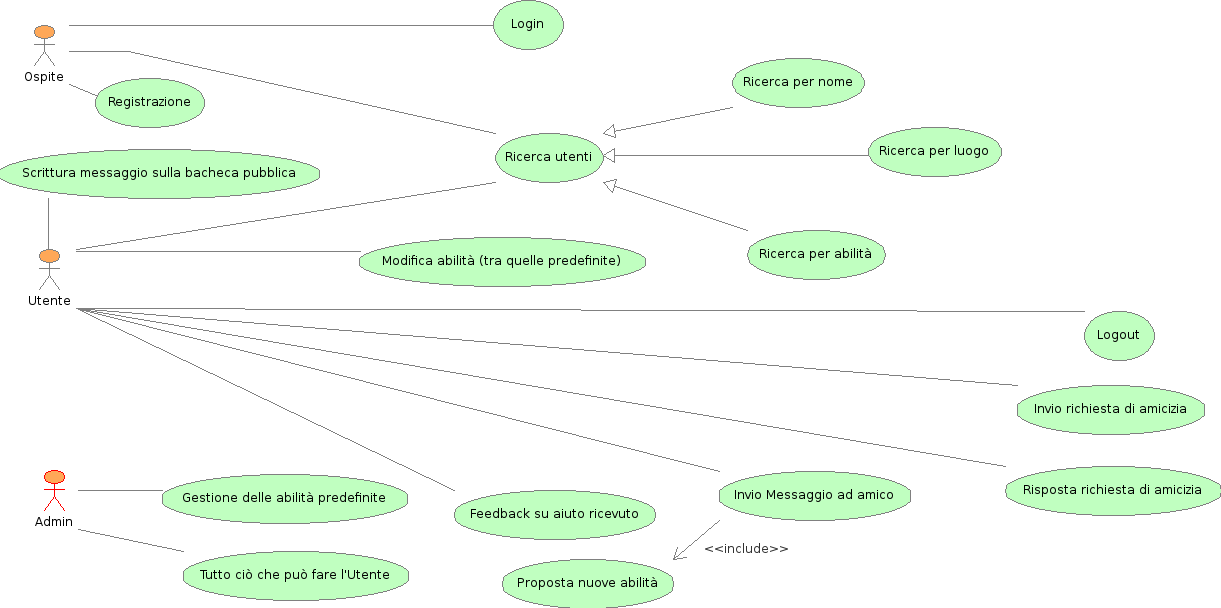
\includegraphics[scale=0.5]{UseCase.png} \\
\caption{\label{Case Diagram} Grafico rappresentante gli attori e i possibili casi d'uso}
\end{figure}

\subsubsection{Tabelle casi d'uso}
\arrayrulecolor{cyan}
\setlength\arrayrulewidth{0.8mm}
\begin{tabularx}{\textwidth}{|c|X|}
\rowcolor[gray]{.9}\hline \textbf{Nome del caso} & Un utente si registra \\ 
\rowcolor[gray]{.9}\hline \textbf{Attori} & Ospite \\ 
\rowcolor[gray]{.9}\hline \textbf{Condizione di entrata} & L'ospite clicca sul pulsante “Registrati” \\ 
\rowcolor[gray]{.9}\hline\raisebox{-27ex}[0pt][0pt]{\textbf{Flusso degli eventi}}& 
\begin{enumerate}
\itemsep0em 
\item L'ospite inserisce negli appositi campi nome, cognome, città, il suo indirizzo mail e la sua password (quest' ultima scelta sul momento).
\item L'ospite seleziona dal set predefinito le abilità che ritiene di possedere.
\item L'ospite clicca sul pulsante di conferma.
\item Il sistema effettua apposite query sul database per verificare che non esista già la mail indicata ed esegue un controllo sulla password per verificare che abbia la lunghezza minima e contenga solo caratteri permessi.
\item Il sistema inserisce nel database i dati del neo-utente ma non mette il flag nel campo corrispondente all'attributo “confermato”
\item Il sistema invia una mail all'indirizzo fornito dall'utente con un link di conferma.
\item L'utente apre la mail e clicca sul link di conferma.
\item Il sistema mette il flag nel campo di cui sopra.
\item Il sistema mostra la pagina di avvenuta registrazione (il login comunque non è ancora stato effettuato).
\end{enumerate}
 \\ 
\rowcolor[gray]{.85}\hline\raisebox{-1ex}[0pt][0pt]{ \textbf{Condizione di uscita}} & Il sistema ha mostrato la pagina di avvenuta registrazione \\
\rowcolor[gray]{.85}\hline\raisebox{-5.5ex}[0pt][0pt] {\textbf{Eccezioni}} & 
\begin{enumerate}
\itemsep0em 
\item La mail inserita dall'utente esiste già nel database
\item La password è lunga meno di 8 caratteri o contiene caratteri diversi da lettere, numeri o underscore.
\end{enumerate}
\\
\hline 
\end{tabularx}
\clearpage
\begin{tabularx}{\textwidth}{|c|X|} 
\rowcolor[gray]{.9}\hline \textbf{Nome del caso} & Un ospite effettua il login \\
\rowcolor[gray]{.9}\hline \textbf{Attori} & Ospite \\ 
\rowcolor[gray]{.9}\hline \textbf{Condizione di entrata} & L'ospite clicca sul pulsante “Login” \\
\rowcolor[gray]{.9}\hline \raisebox{-10ex}[0pt][0pt]{\textbf{Flusso degli eventi}} & 
\begin{enumerate}
\itemsep0em 
\item L'ospite inserisce negli appositi campi mail e password.
\item L'ospite preme il pulsante di conferma.
\item Il sistema effettua una query nel database con i dati inseriti e, in caso la query ritorni un valore non vuoto, visualizza la pagina personale dell'utente corrispondente.
\end{enumerate}
 \\ 
\rowcolor[gray]{.9}\hline \textbf{Condizione di uscita} & L'utente si trova nella sua pagina personale \\
\rowcolor[gray]{.9}\hline \textbf{Eccezioni} & La query del sistema ritorna null
\\
\hline 
\end{tabularx} \\[3\baselineskip]
\begin{tabularx}{\textwidth}{|c|X|}
\rowcolor[gray]{.9}\hline  \textbf{Nome del caso} & Un utente modifica il proprio set di abilità \\
\rowcolor[gray]{.9}\hline  \textbf{Attori} & Utente \\ 
\rowcolor[gray]{.9}\hline \raisebox{-1ex}[0pt][0pt]{ \textbf{Condizione di entrata}} & L'utente clicca sul pulsante di modifica del set di abilità presente nella sua home \\
\rowcolor[gray]{.9}\hline \raisebox{-11ex}[0pt][0pt]{ \textbf{Flusso degli eventi}} & 
\begin{enumerate}
\itemsep0em 
\item L'utente eventualmente (non è obligato a farlo) toglie il flag da una o più abilità che ha e mette il flag su una o più nuove abilità. (Non c'è limite al numero di abilità possedibili ed è possibile avere zero abilità)
\item L'utente clicca sul pulsante di conferma.
\item Il sistema aggiorna il database
\item Il sistema notifica all'utente il successo dell'operazione e lo reindirizza alla sua pagina personale
\end{enumerate}
 \\ 
\rowcolor[gray]{.9}\hline \raisebox{-1ex}[0pt][0pt]{ \textbf{Condizione di uscita}} & L'utente si ritrova nella sua pagina personale e il suo set è modificato correttamente \\
\rowcolor[gray]{.9}\hline \raisebox{-2ex}[0pt][0pt]{ \textbf{Eccezioni}} & Nessuna: gli unici errori possono essere dovuti a guasti non deterministici della macchina o a cadute della connessione internet
\\
\hline 
\end{tabularx} \clearpage
\begin{tabularx}{\textwidth}{|c|X|}
\rowcolor[gray]{.9}\hline  \raisebox{-1ex}[0pt][0pt]{\textbf{Nome del caso}} & Un ospite tenta di pubblicare una richiesta di aiuto in una categoria\\
\rowcolor[gray]{.9}\hline  \textbf{Attori} & Ospite \\ 
\rowcolor[gray]{.9}\hline \raisebox{-1ex}[0pt][0pt]{ \textbf{Condizione di entrata}} & L' ospite clicca sul pulsante “Inserisci messaggio” presente sulla bacheca pubblica \\
\rowcolor[gray]{.9}\hline  \raisebox{-5.5ex}[0pt][0pt]{\textbf{Flusso degli eventi}} & 
\begin{enumerate}
\itemsep0em 
\item Il sistema risponde con un popup
\item L' ospite legge il contenuto del popup e clicca sul pulsante ok per chiuderlo
\end{enumerate}
 \\ 
\rowcolor[gray]{.9}\hline \textbf{Condizione di uscita} & L'ospite si ritrova nella pagina della categoria \\
\rowcolor[gray]{.9}\hline \textbf{Eccezioni} & Nessuna, vedi caso precedente
\\
\hline 
\end{tabularx} \\[3\baselineskip]
\begin{tabularx}{\textwidth}{|c|X|}
\rowcolor[gray]{.9}\hline  \raisebox{-1ex}[0pt][0pt]{\textbf{Nome del caso}} & Un utente pubblica una richiesta di aiuto sulla bacheca pubblica \\
\rowcolor[gray]{.9}\hline  \textbf{Attori} & Utente \\ 
\rowcolor[gray]{.9}\hline \raisebox{-1ex}[0pt][0pt]{ \textbf{Condizione di entrata}} & L' utente clicca sul pulsante “Inserisci messaggio” presente sulla bacheca pubblica \\
\rowcolor[gray]{.9}\hline  \raisebox{-8ex}[0pt][0pt]{\textbf{Flusso degli eventi}} & 
\begin{enumerate}
\itemsep0em 
\item L utente compone il messaggio
\item L' utente clicca sul pulsante di pubblicazione del messaggio
\item Il sistema fa in modo che il messaggio diventi visibile a chiunque
\end{enumerate}
 \\ 
\rowcolor[gray]{.9}\hline \textbf{Condizione di uscita} & Il messaggio è visibile in bacheca \\
\rowcolor[gray]{.9}\hline \textbf{Eccezioni} & Nessuna
\\
\hline 
\end{tabularx} \\[1\baselineskip]
\begin{tabularx}{\textwidth}{|c|X|}
\rowcolor[gray]{.9}\hline  \raisebox{-1ex}[0pt][0pt]{\textbf{Nome del caso}} & Un ospite effettua una ricerca su tutto l'insieme di utenti di SWIM \\
\rowcolor[gray]{.9}\hline  \textbf{Attori} & Ospite \\ 
\rowcolor[gray]{.9}\hline  \textbf{Condizione di entrata} & L'ospite clicca sul pulsante di ricerca \\
\rowcolor[gray]{.9}\hline \raisebox{-10ex}[0pt][0pt]{ \textbf{Flusso degli eventi}} & 
\begin{enumerate}
\itemsep0em 
\item L'ospite riempie almeno uno dei seguenti campi: “nome e cognome”, “città” e/o seleziona almeno un'abilità dalla scroll-list.
\item L'ospite clicca sul pulsante di conferma.
\item Il sistema effettua una query con i dati ricevuti.
\item Il sistema mostra una finestra con una lista (eventualmente vuota) di risultati
\end{enumerate}
 \\ 
\rowcolor[gray]{.9}\hline  \textbf{Condizione di uscita} & La finestra dei risultati è visibile \\
\rowcolor[gray]{.9}\hline  \raisebox{-4ex}[0pt][0pt]{\textbf{Eccezioni} }&
\begin{enumerate}
\itemsep0em
\item Viene effettuata una ricerca senza parametri.
\item I dati inseriti contengono caratteri non consentiti.
\end{enumerate}
\\
\hline 
\end{tabularx} \\[2\baselineskip]
\begin{tabularx}{\textwidth}{|c|X|}
\rowcolor[gray]{.9}\hline \raisebox{-1ex}[0pt][0pt]{ \textbf{Nome del caso}} & Un utente chiede ad un amministratore di aggiungere una nuova abilità al set predefinito di sistema \\
\rowcolor[gray]{.9}\hline  \textbf{Attori} & Utente, Amministratore \\ 
\rowcolor[gray]{.9}\hline \raisebox{-1ex}[0pt][0pt]{ \textbf{Condizione di entrata}} & L'utente clicca sul pulsante “Invia messaggio” dal profilo pubblico dell'amministratore \\
\rowcolor[gray]{.9}\hline  \raisebox{-10ex}[0pt][0pt]{\textbf{Flusso degli eventi}} & 
\begin{enumerate}
\itemsep0em
\item L'utente compone il corpo del messaggio includendo una chiara descrizione della nuova abilità, il suo nome e le motivazioni per cui ha proposto di aggiungerla.
\item L'utente clicca sul pulsante di invio messaggio.
\item Il sistema invia il messaggio all'amministratore e fa comparire una notifica sulla sua pagina personale.
\end{enumerate}
 \\ 
\rowcolor[gray]{.9}\hline  \raisebox{-1ex}[0pt][0pt]{\textbf{Condizione di uscita}} & Il messaggio è inviato correttamente e sulla pagina dell'amministratore compare una notifica \\
\rowcolor[gray]{.9}\hline  \textbf{Eccezioni} & Nessuna
\\
\hline 
\end{tabularx} \\[3\baselineskip]
\begin{tabularx}{\textwidth}{|c|X|}
\rowcolor[gray]{.9}\hline \raisebox{-1ex}[0pt][0pt]{ \textbf{Nome del caso}} & Un utente invia una richiesta di amicizia ad un altro utente senza passare dai suggerimenti \\
\rowcolor[gray]{.9}\hline  \textbf{Attori} & Utente A, Utente B \\ 
\rowcolor[gray]{.9}\hline \raisebox{-1ex}[0pt][0pt]{ \textbf{Condizione di entrata}} & L'utente A clicca sul pulsante “Aggiungi” dalla pagina pubblica dell'utente B \\
\rowcolor[gray]{.9}\hline  \raisebox{-1ex}[0pt][0pt]{\textbf{Flusso degli eventi}} & Il sistema notifica all'utente B che l'utente A gli ha inviato una richiesta di amicizia.
 \\ 
\rowcolor[gray]{.9}\hline  \textbf{Condizione di uscita} & All'utente B è arrivata la notifica \\
\rowcolor[gray]{.9}\hline  \textbf{Eccezioni} & Nessuna
\\
\hline 
\end{tabularx} \\[3\baselineskip]

\begin{tabularx}{\textwidth}{|c|X|}
\rowcolor[gray]{.9}\hline \raisebox{-1ex}[0pt][0pt]{ \textbf{Nome del caso}} & Un utente risponde positivamente ad una richiesta di amicizia \\
\rowcolor[gray]{.9}\hline  \textbf{Attori} & Utente C, Utente D \\ 
\rowcolor[gray]{.9}\hline  \raisebox{-1ex}[0pt][0pt]{\textbf{Condizione di entrata}} & L'utente C clicca su “Conferma” dalla notifica della richiesta \\
\rowcolor[gray]{.9}\hline  \raisebox{-5.5ex}[0pt][0pt]{\textbf{Flusso degli eventi}} & 
\begin{enumerate}
\itemsep0em 
\item Il sistema aggiunge D agli amici di C e viceversa.
\item Il sistema notifica C del buon fine dell'azione e D del fatto che C abbia accettato la sua richiesta.
\end{enumerate}
 \\ 
\rowcolor[gray]{.9}\hline  \textbf{Condizione di uscita} & Le notifiche sono state spedite agli utenti coinvolti \\
\rowcolor[gray]{.9}\hline  \textbf{Eccezioni}& Nessuna
\\
\hline 
\end{tabularx}
\clearpage
\begin{tabularx}{\textwidth}{|c|X|}
\rowcolor[gray]{.9}\hline  \textbf{Nome del caso} & Un utente dà un feedback \\
\rowcolor[gray]{.9}\hline  \textbf{Attori} & Utente A, Utente B \\ 
\rowcolor[gray]{.9}\hline  \raisebox{-1ex}[0pt][0pt]{\textbf{Condizione di entrata}} & L'utente A ha ricevuto un messaggio di risposta dall'utente B \\
\rowcolor[gray]{.9}\hline  \raisebox{-12ex}[0pt][0pt]{\textbf{Flusso degli eventi}} & 
\begin{enumerate}
\itemsep0em 
\item L'utente A clicca sul pulsante “Dai feedback” contenuto nel messaggio di risposta di B.
\item L'utente A seleziona il livello del feedback (da 1 a 10) dal popup che il sistema ha aperto
\item L'utente clicca su “Conferma”.
\item Il sistema notifica B del feedback ricevuto con un messaggio automatico e aggiorna la media dei suoi feedback.
\end{enumerate}
 \\ 
\rowcolor[gray]{.9}\hline  \textbf{Condizione di uscita} & La media è correttamente aggiornata \\
\rowcolor[gray]{.9}\hline  \textbf{Eccezioni} & Nessuna
\\
\hline 
\end{tabularx} \\[3\baselineskip]
\begin{tabularx}{\textwidth}{|c|X|}
\rowcolor[gray]{.9}\hline  \textbf{Nome del caso} & Un utente cancella il proprio account \\
\rowcolor[gray]{.9}\hline  \textbf{Attori} & Utente \\ 
\rowcolor[gray]{.9}\hline  \raisebox{-1ex}[0pt][0pt]{\textbf{Condizione di entrata}} & L'utente preme il pulsante “Cancella account” dalla propria pagina personale \\
\rowcolor[gray]{.9}\hline  \raisebox{-12ex}[0pt][0pt]{\textbf{Flusso degli eventi}} & 
\begin{enumerate}
\itemsep0em
\item L'utente conferma la volontà di cancellazione dal popup che il sistema apre.
\item Il sistema slogga l'utente, cancella tutti i suoi legami di amicizia (il che vuol dire che rimuove tutti i suoi amici e dalle loro liste di amici rimuove l'utente stesso) e cancella i suoi dati dal database.
\item Il sistema notifica con un popup l'avvenuta cancellazione e reindirizza alla pagina principale di SWIM.
\end{enumerate}
 \\ 
\rowcolor[gray]{.9}\hline  \textbf{Condizione di uscita} & Il sistema ha notificato l'avvenuta cancellazione \\
\rowcolor[gray]{.9}\hline  \textbf{Eccezioni} & Nessuna
\\
\hline 
\end{tabularx}
\clearpage
\vspace*{10cm}
\section{Modelli UML}
\subsection{Sequence diagrams}
\begin{figure}
\centering
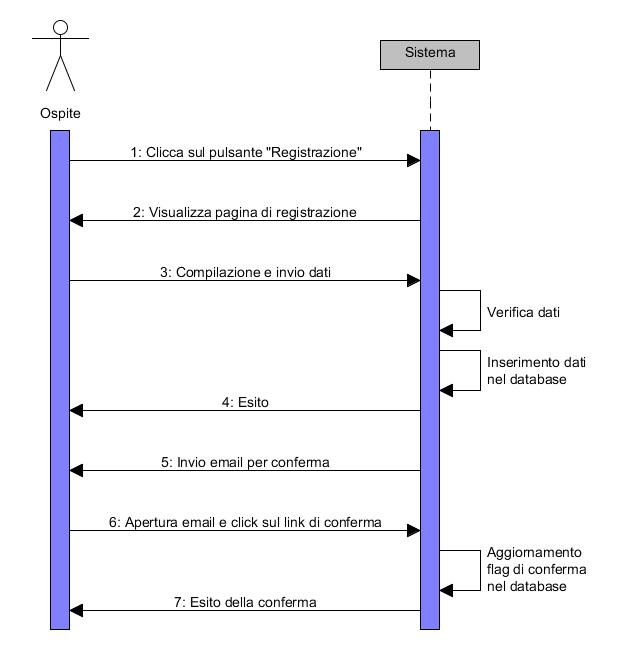
\includegraphics[scale=0.70]{sDiagrams/creazioneUtente.jpg}
\caption{\label{creazioneUtente} Creazione di un utente}
\vspace{1cm}
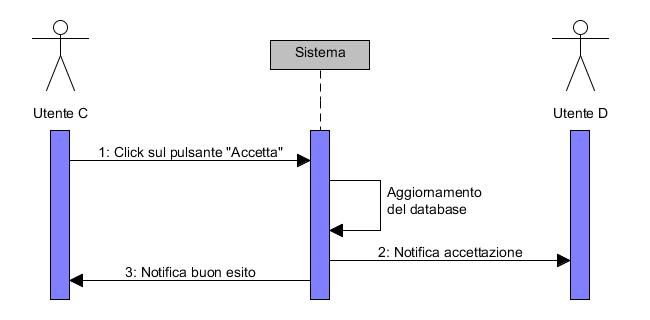
\includegraphics[scale=0.70]{sDiagrams/accettazioneAmicizia.jpg} \\
\caption{\label{accettazioneAmicizia} Accettazione di una richiesta di amicizia}
\end{figure}
\clearpage
\begin{figure}
\centering
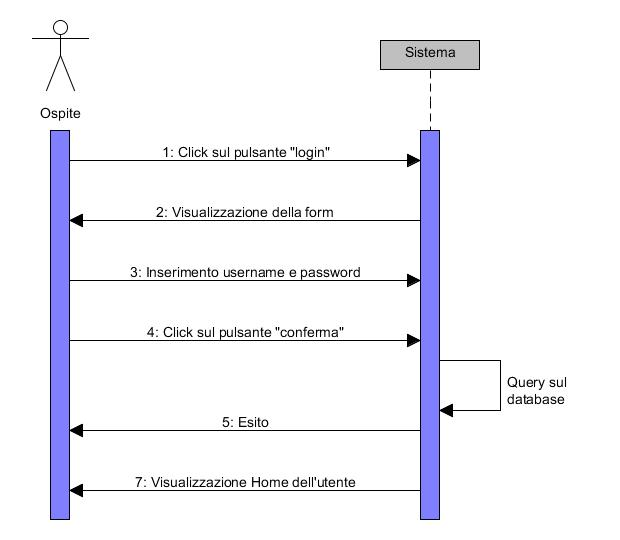
\includegraphics[scale=0.70]{sDiagrams/login.jpg} \\
\caption{\label{login} Login di un utente}
\vspace{0.5cm}
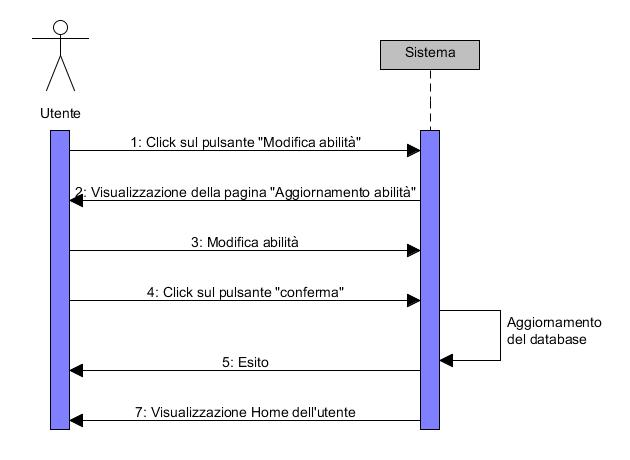
\includegraphics[scale=0.70]{sDiagrams/modificaAbilita.jpg} \\
\caption{\label{modificaAbilita} Modifica del set di abilità}
\end{figure}
\clearpage
\begin{figure}
\centering
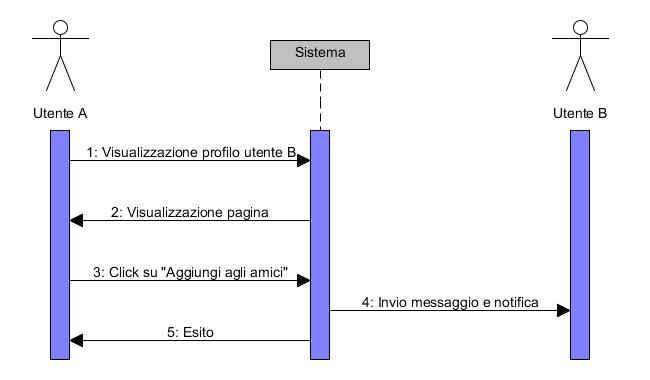
\includegraphics[scale=0.70]{sDiagrams/richiestaAmicizia.jpg} \\
\caption{\label{richiestaAmicizia} Invio di una richiesta di amicizia}
\vspace{2cm}
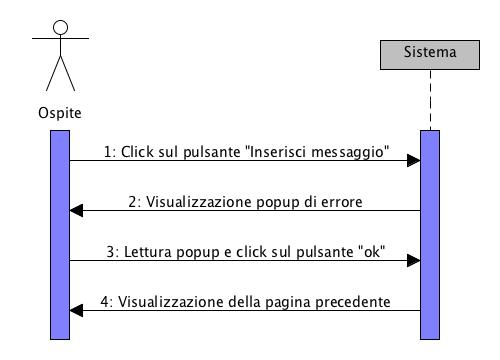
\includegraphics[scale=0.70]{sDiagrams/tentativoCreazioneThread.jpg} \\
\caption{\label{tentativoCreazioneThread} Un ospite tenta di creare un thread}
\end{figure}
\begin{figure}
\centering
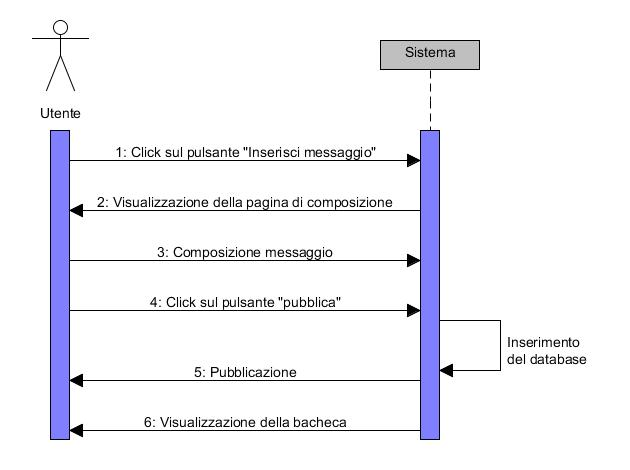
\includegraphics[scale=0.70]{sDiagrams/creazioneThread.jpg} \\
\caption{\label{creazioneThread} Invio di un nuovo messaggio sulla bacheca pubblica}
\vspace{0.5cm}
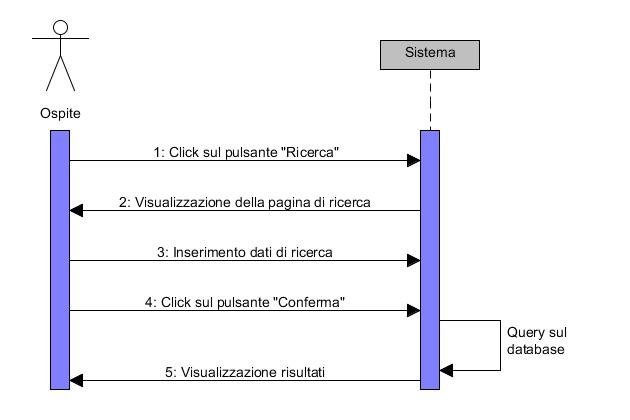
\includegraphics[scale=0.70]{sDiagrams/ricercaUtenti.jpg} \\
\caption{\label{ricercaUtenti} Ricerca di un utente}
\end{figure}
\begin{figure}
\centering
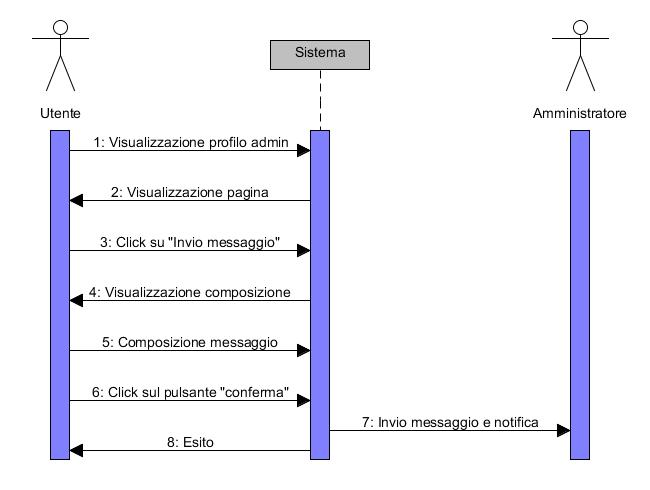
\includegraphics[scale=0.70]{sDiagrams/invioMessaggio.jpg} \\
\caption{\label{invioMessaggio} Invio di un messaggio privato}
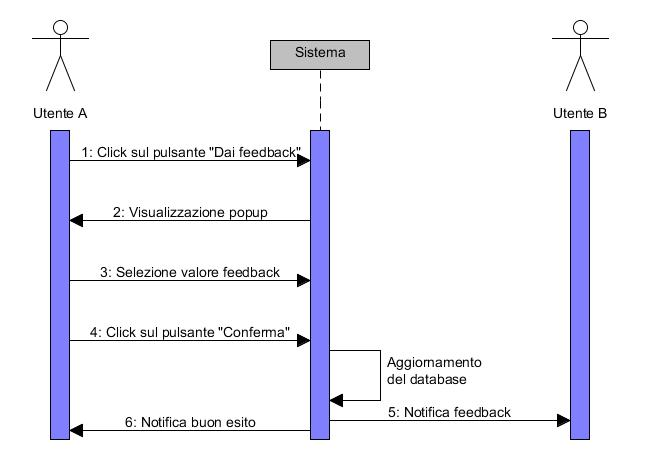
\includegraphics[scale=0.70]{sDiagrams/invioFeedback.jpg} \\
\caption{\label{invioFeedback} Invio di un feedback}
\end{figure}
\begin{figure}
\centering
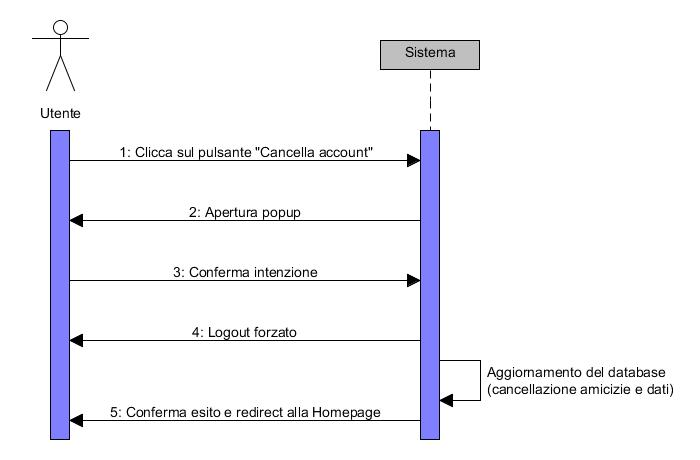
\includegraphics[scale=0.70]{sDiagrams/cancellazioneAccount.jpg} \\
\caption{\label{cancellazioneAccount} Cancellazione dell'account}
\end{figure}
\clearpage
\subsection{Statechart}
Con i seguenti statechart abbiamo controllato il flusso delle operazioni del sistema in alcuni casi specifici: \\[1\baselineskip]
\textit{1. Invio del feedback dopo l’aiuto ricevuto}: \\
\begin{center}
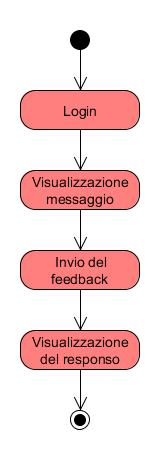
\includegraphics[scale=0.75]{statechart/invioFeedback.jpg} \\
\end{center}
\clearpage
\textit{2. Inserimento di una risposta ad un messaggio}: \\
\begin{center}
\includegraphics[scale=0.75]{statechart/InvioRispostaMessaggio.jpg} \\

\end{center}
\clearpage
\section{Modello Alloy}
\subsection{Signatures}
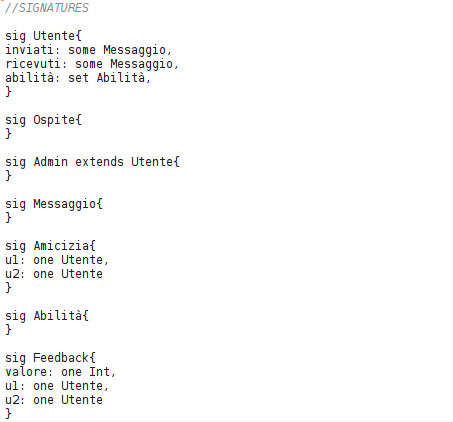
\includegraphics[scale=0.6]{signatures.png}
\subsection{Facts}
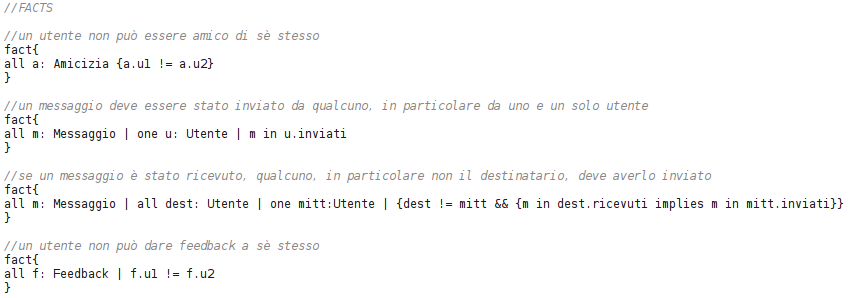
\includegraphics[scale=0.6]{facts.png} \\
\clearpage
\section{Strumenti utilizzati}
\begin{enumerate}
\itemsep0em
\item \textbf{\LaTeX}: TeXstudio, Kile e MacTeX
\item \textbf{Alloy Analizer 4.2}: per la gestione delle specifiche scritte in Alloy
\item \textbf{Umlet e Umbrello}: per la gestione dei grafici e dei diagrammi UML
\end{enumerate}

\section{Rettifiche in corso d'opera}
A causa della mancanza di tempo, che tra le cause principali presenta ritardi dovuti alla difficoltà di configurare l'ambiente di lavoro, alcune funzionalità che non erano strettamente richieste dalla specifica non sono state introdotte nell'applicazione.
\begin{itemize}
\item [$\textcolor{red}{\star}$]Non sono presenti thread, categorie e quindi tutto ciò che era implicato alla parte pubblica del sistema: si potrà interagire con gli altri utenti tramite l'invio dei soli messaggi privati e gli ospiti potranno effettuare solamente delle ricerche.

\item[$\textcolor{red}{\star}$]Non è possibile proporre attivamente nuove amicizie agli altri utenti, la funzionalità di richiesta o accettazione di un' amicizia è comunque presente e funziona regolarmente

\item[$\textcolor{red}{\star}$]Una volta entrati non sarà possibile eliminare il propio profilo, SWIM è una prigione!
\end{itemize}


\end{document}